%% Wind Tunnel — Figure Captions
%% Five panels. Include this file after \usepackage{graphicx} in the main document,
%% or paste individual figure* environments directly into windtunnel-code-testing.tex.

% ─────────────────────────────────────────────────────────────────────────────
\begin{figure*}[!htbp]
    \centering
    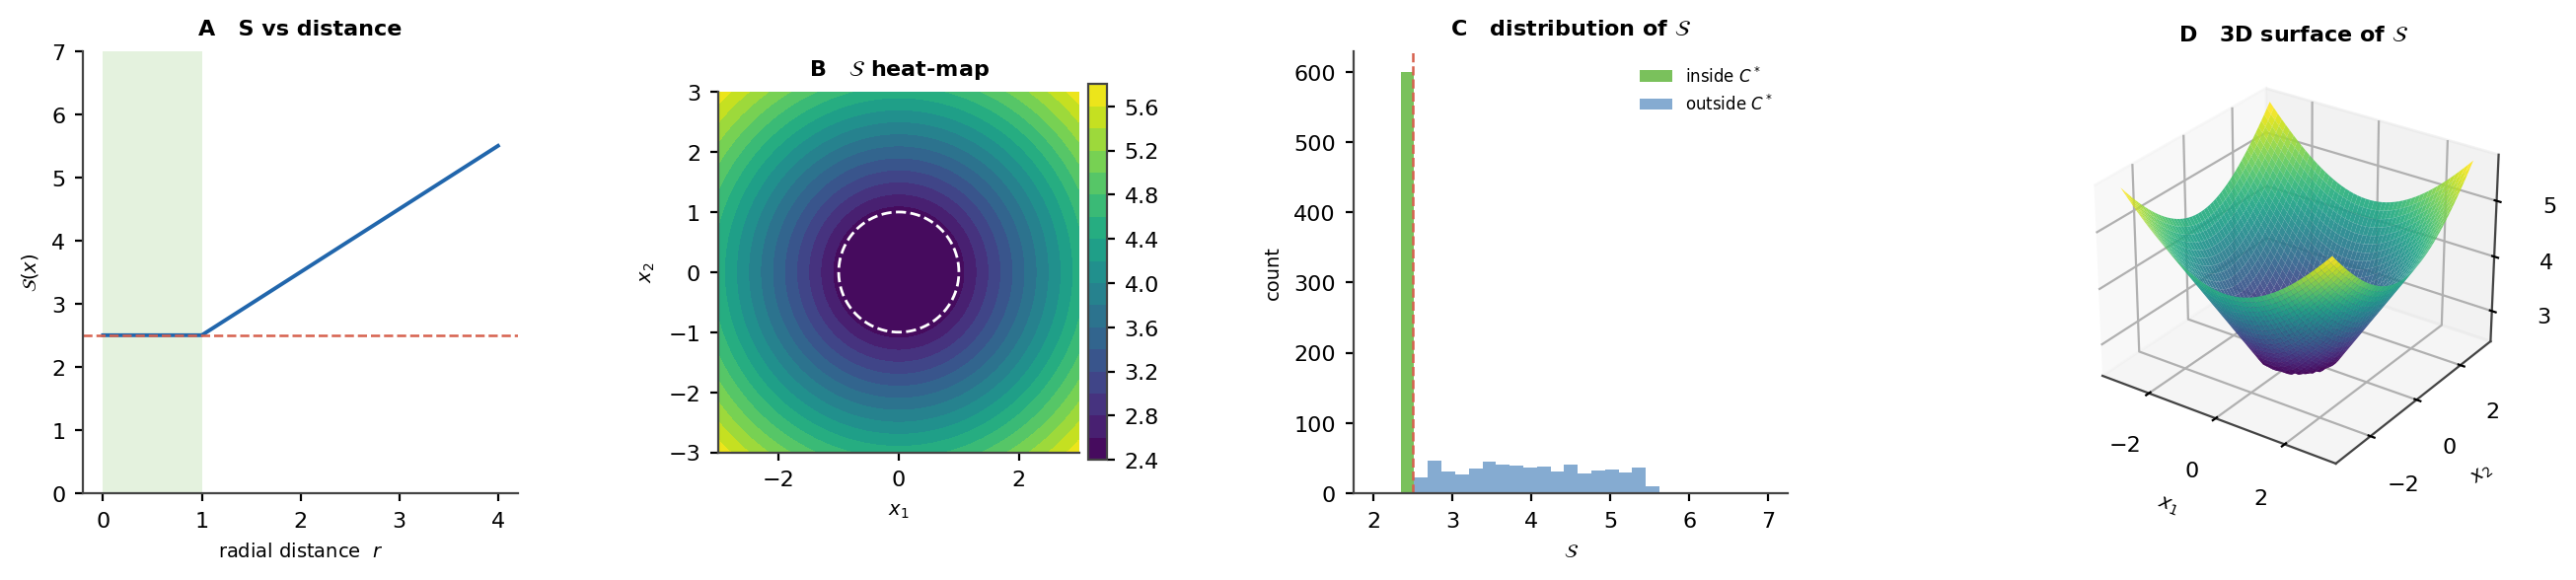
\includegraphics[width=\textwidth]{figures/panel_1.png}
    \caption{\textbf{Semantic Entropy $\mathcal{S}$ and the Action-Cell $C^*$.}
    (\textbf{A})~$\mathcal{S}(x)$ on the linear $y$-axis versus radial distance
    $r = \|x - c^*\|$ from the cell centre on the $x$-axis.  The shaded band
    marks the interior $r \leq R$ (action-cell $C^*$, seagreen); inside, entropy
    is constant at the floor $\mathcal{S}_\flat$ (red dashed), confirming
    Axiom~\ref{ax:floor} (Floor Positivity).  Outside the cell, $\mathcal{S}$
    grows linearly with distance, as required by Axiom~\ref{ax:monotone}
    (Monotonicity).
    (\textbf{B})~Two-dimensional filled-contour map of $\mathcal{S}(x_1, x_2)$
    in outcome space.  Colour encodes entropy magnitude (dark = low, bright =
    high); the white dashed circle is the boundary of $C^*$.  The flat floor
    region inside the circle and the monotone ascent outside are visible
    simultaneously, illustrating Definition~\ref{def:action-cell}.
    (\textbf{C})~Histogram of $\mathcal{S}$ values sampled uniformly inside
    $C^*$ (seagreen) and uniformly outside $C^*$ (blue).  All interior samples
    pile at $\mathcal{S}_\flat$ (red dashed); exterior samples spread above it.
    Confirms that the cell is the unique minimum-entropy region and that
    Axiom~\ref{ax:continuity} (Lipschitz Continuity) holds: no exterior sample
    reaches the floor.
    (\textbf{D})~Three-dimensional surface of $\mathcal{S}(x_1, x_2)$.  The
    flat plateau at height $\mathcal{S}_\flat$ is the action-cell; the surface
    rises in every direction outside it.  The bowl-free plateau geometry makes
    visible why truth is a positive-volume region rather than a point
    (Definition~\ref{def:action-cell}): all states on the plateau are
    indistinguishable by $\mathcal{S}$.}
    \label{fig:panel1-s-entropy}
\end{figure*}

% ─────────────────────────────────────────────────────────────────────────────
\begin{figure*}[!htbp]
    \centering
    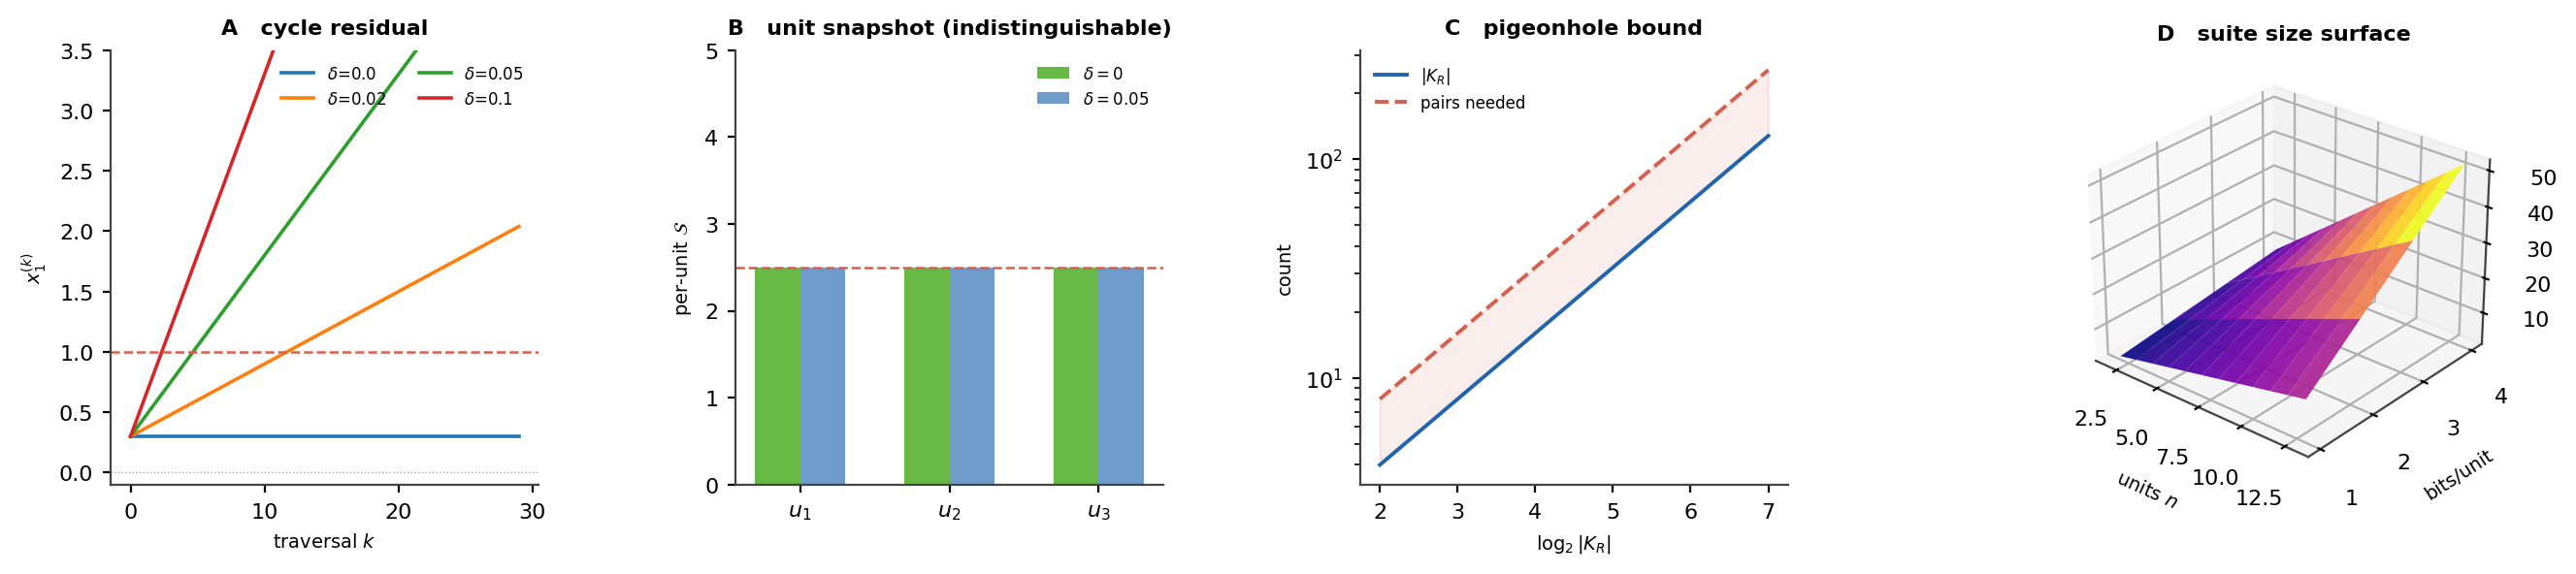
\includegraphics[width=\textwidth]{figures/panel_2.png}
    \caption{\textbf{Local Invisibility and the No Template Bound.}
    (\textbf{A})~Cycle residual $x_1^{(k)} = x_0 + 3k\delta$ on the $y$-axis
    versus traversal count $k$ on the $x$-axis for four per-edge drift values
    $\delta \in \{0, 0.02, 0.05, 0.10\}$.  The red dashed line marks the
    action-cell boundary.  For $\delta > 0$ the trajectory exits $C^*$ after
    finitely many traversals; for $\delta = 0$ it never moves.  This is the
    explicit witness constructed in the proof of
    Theorem~\ref{thm:local-invisibility} (Local Invisibility Theorem): each
    individual unit remains in $[0,1]$ throughout, yet the cycle accumulates
    global semantic error.
    (\textbf{B})~Per-unit semantic entropy $\mathcal{S}$ at traversal $k=0$
    for the two cases $\delta=0$ (seagreen) and $\delta=0.05$ (blue) across
    units $u_1, u_2, u_3$.  Both bars reach the same height at $\mathcal{S}_\flat$
    (red dashed): unit-level observation is completely uninformative about the
    cycle-level drift.  Empirical content of
    Corollary~\ref{cor:unit-test-blind}: unit tests are blind to this failure
    class.
    (\textbf{C})~Observer capacity $|K_R|$ (solid blue) and the number of
    boundary pairs that must be distinguished (dashed red) versus
    $\log_2|K_R|$ on the $x$-axis (log $y$-axis).  The red curve grows faster
    than the blue: whenever $\kappa(S) > \log_2|K_R|$ the pigeonhole gap opens,
    and no function stored in $R$ can decide $C^*$-membership.  Direct
    empirical support for Theorem~\ref{thm:no-template} (No Template Theorem).
    (\textbf{D})~Three-dimensional surface of $\log_2$(required test-suite
    size) over the grid of unit count $n$ ($x$-axis) and bits per unit
    ($y$-axis).  The surface is superlinear in both axes; for modest $n$ and
    bit-depths the suite size already exceeds any practical bound.  Quantifies
    Corollary~\ref{cor:test-suite-incomplete}: every test suite of bounded
    complexity is an incomplete specification of $C^*$.}
    \label{fig:panel2-invisibility-template}
\end{figure*}

% ─────────────────────────────────────────────────────────────────────────────
\begin{figure*}[!htbp]
    \centering
    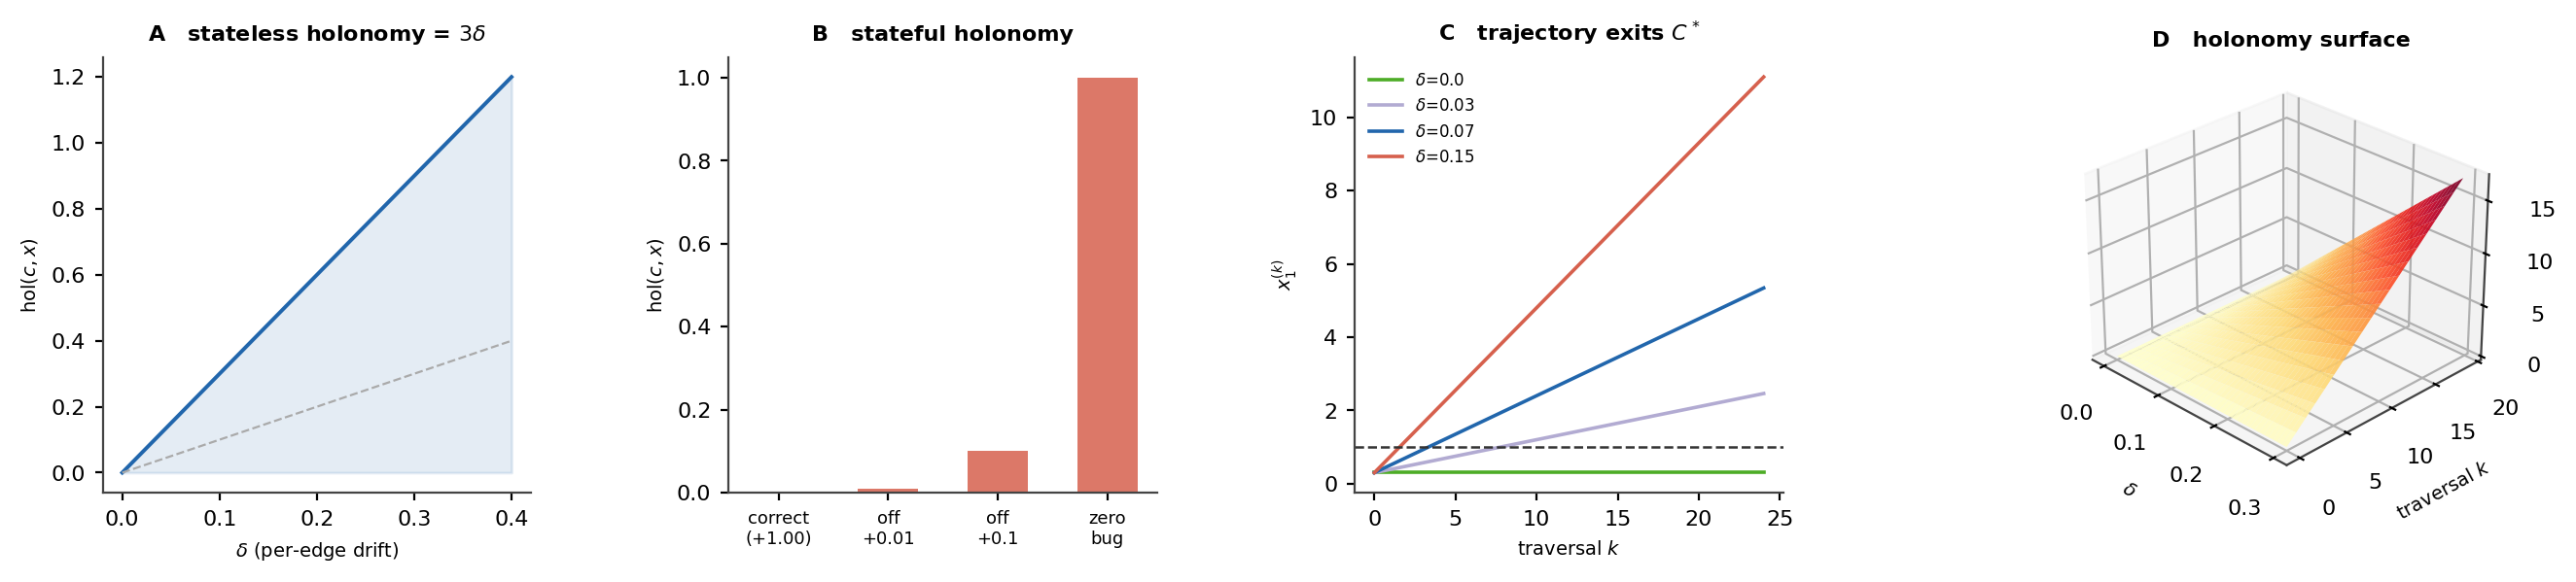
\includegraphics[width=\textwidth]{figures/panel_3.png}
    \caption{\textbf{Holonomy and Cycle Inconsistency.}
    (\textbf{A})~Stateless holonomy $\hol(c, x) = 3\delta$ on the $y$-axis
    versus per-edge drift $\delta$ on the $x$-axis.  The relationship is
    exactly linear with slope equal to the cycle length (here $|c|=3$).  The
    grey dotted diagonal is the identity $\hol = \delta$.  This confirms that
    even a small per-edge drift compounds multiplicatively around the cycle,
    consistent with Definition~\ref{def:holonomy}:
    $\hol(c,x) = \|T_c(x) - T_c^{\mathrm{spec}}(x)\|$.
    (\textbf{B})~Stateful holonomy as a bar chart: four accumulator variants
    (correct $+1.00$, off-by-$0.01$, off-by-$0.1$, zero-bug) on the $x$-axis,
    $\hol(c, x)$ on the $y$-axis.  The correct implementation yields
    $\hol = 0$ (seagreen); each erroneous variant yields a positive bar
    (crimson).  Illustrates that holonomy detects semantic deviation from the
    declared cycle specification $T_c^{\mathrm{spec}}$, not merely deviation
    from the identity --- the corrected definition that avoids condemning
    legitimate stateful loops.
    (\textbf{C})~State trajectory $x_1^{(k)}$ on the $y$-axis versus traversal
    $k$ on the $x$-axis for four drift values.  The black dashed line is the
    cell boundary.  For any $\delta > 0$, the trajectory eventually exits
    $C^*$; for $\delta = 0$ it is constant.  Supplies the constructive half of
    Theorem~\ref{thm:hac} (Cycle Inconsistency Theorem): nonzero holonomy
    produces a trajectory that necessarily exits the action-cell.
    (\textbf{D})~Three-dimensional holonomy surface over the grid of
    per-edge drift $\delta$ ($x$-axis) and traversal count $k$ ($y$-axis),
    with accumulated holonomy $3\delta k$ on the $z$-axis.  The surface rises
    without bound as either axis grows, confirming that cycle-level semantic
    error is not self-correcting: it accumulates monotonically with repeated
    traversal.}
    \label{fig:panel3-holonomy}
\end{figure*}

% ─────────────────────────────────────────────────────────────────────────────
\begin{figure*}[!htbp]
    \centering
    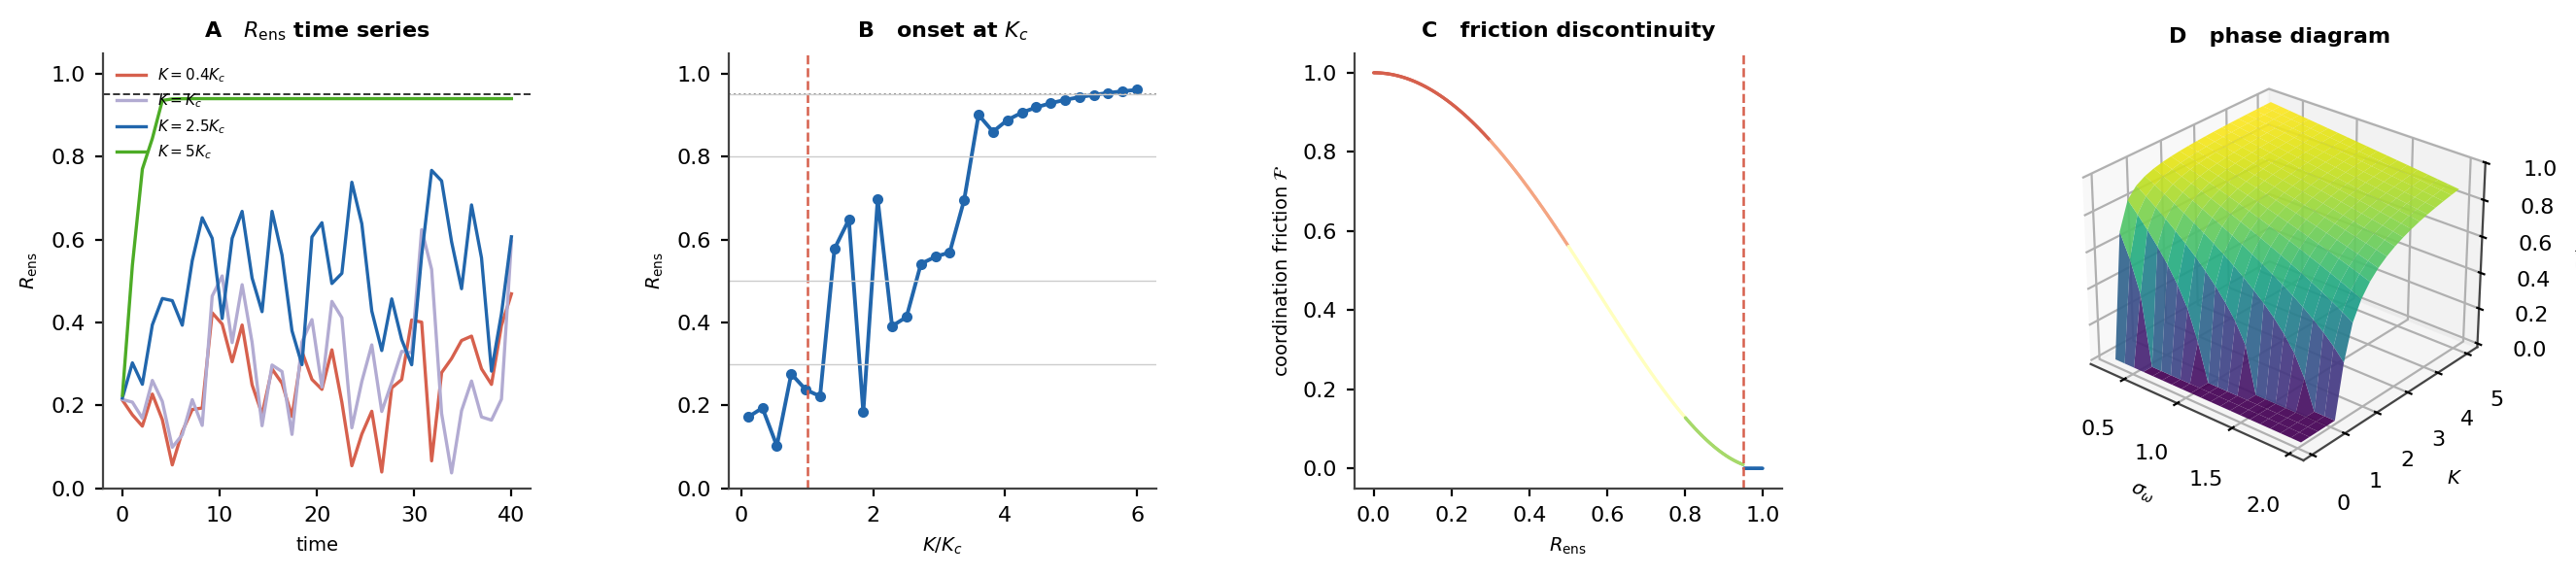
\includegraphics[width=\textwidth]{figures/panel_4.png}
    \caption{\textbf{Kuramoto Dynamics and the Five Coordination Regimes.}
    (\textbf{A})~Ensemble order parameter $R_\mathrm{ens}(t)$ on the $y$-axis
    versus time on the $x$-axis for four coupling strengths $K \in
    \{0.4, 1.0, 2.5, 5.0\} \times K_c$.  The black dashed line at
    $R_\mathrm{ens} = 0.95$ marks the Coherent/Phase-locked boundary
    (Definition~\ref{def:regimes}).  At $K < K_c$ the order parameter
    fluctuates near zero (turbulent regime); at $K = K_c$ it begins to
    climb; at $K = 5K_c$ it reaches and holds $R_\mathrm{ens} \approx 1$.
    Empirical content of Definition~\ref{def:kuramoto}.
    (\textbf{B})~Steady-state $R_\mathrm{ens}$ on the $y$-axis versus
    $K/K_c$ on the $x$-axis (onset curve).  The vertical red dashed line
    marks $K_c = 2\sigma_\omega / \pi$ (Proposition~\ref{prop:critical-coupling}).
    The curve is near-zero for $K < K_c$ and rises sharply above it,
    reproducing the Kuramoto bifurcation.  Horizontal grey lines mark the five
    regime boundaries at $R_\mathrm{ens} \in \{0.30, 0.50, 0.80, 0.95\}$.
    (\textbf{C})~Coordination friction $\mathcal{F}$ on the $y$-axis versus
    $R_\mathrm{ens}$ on the $x$-axis.  Each point is coloured by its
    coordination regime (red = Turbulent, orange = Aperture-dominated,
    yellow = Hierarchical-cascade, green = Coherent, blue = Phase-locked).
    The vertical red dashed line at $R_\mathrm{ens} = 0.95$ shows the
    discontinuous drop of $\mathcal{F}$ to exactly zero --- no intermediate
    state exists.  Direct visualisation of Theorem~\ref{thm:partition-extinction}
    (Partition Extinction).
    (\textbf{D})~Three-dimensional phase diagram: steady-state
    $R_\mathrm{ens}^*$ (mean-field approximation $\sqrt{\max(0,1-K_c/K)}$)
    on the $z$-axis over a grid of frequency spread $\sigma_\omega$ ($x$-axis)
    and coupling $K$ ($y$-axis).  The surface maps the entire
    (disorder, coupling) parameter space to coordination outcome, showing the
    regime frontier as a curved ridge.  At fixed $\sigma_\omega$ the system
    crosses from incoherence to synchrony as $K$ increases; at fixed $K$ wider
    frequency spreads suppress coherence.}
    \label{fig:panel4-kuramoto}
\end{figure*}

% ─────────────────────────────────────────────────────────────────────────────
\begin{figure*}[!htbp]
    \centering
    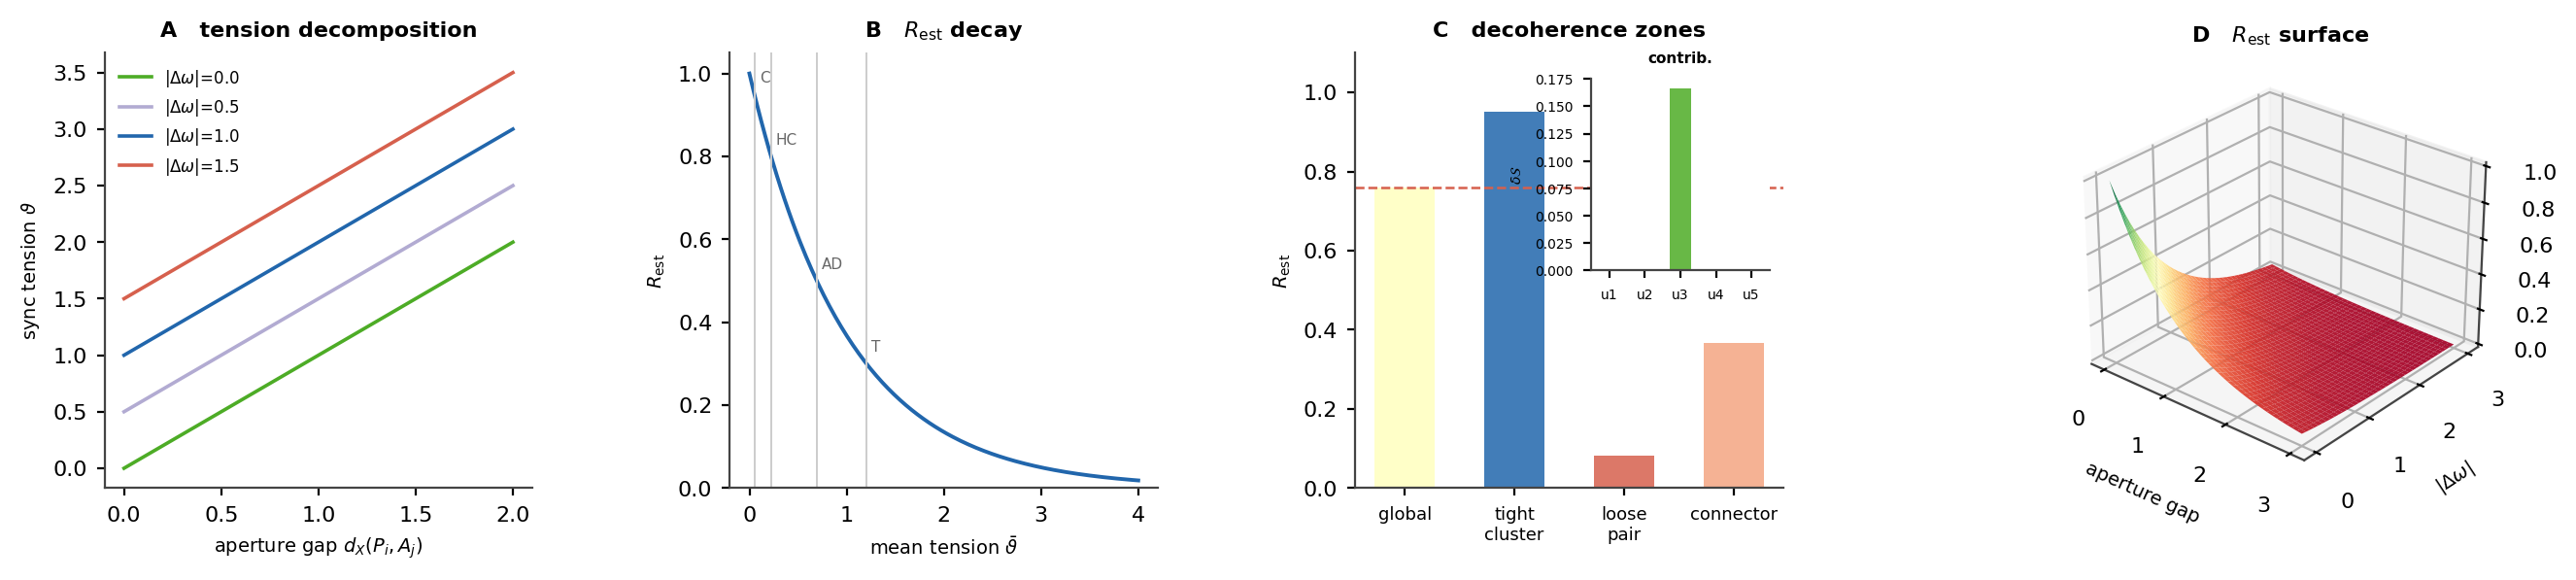
\includegraphics[width=\textwidth]{figures/panel_5.png}
    \caption{\textbf{Synchronisation Tension, Decoherence Zones, and Purposelessness.}
    (\textbf{A})~Synchronisation tension $\vartheta(u_i, u_j) = d_X(P_{u_i},
    A_{u_j}) + |\Delta\omega|$ on the $y$-axis versus aperture gap
    $d_X(P_{u_i}, A_{u_j})$ on the $x$-axis for four frequency-difference
    values $|\Delta\omega| \in \{0, 0.5, 1.0, 1.5\}$.  The linear family of
    curves shows that tension decomposes additively into an aperture term and a
    frequency term (Definition~\ref{def:sync-tension}).  At zero aperture gap,
    tension equals the frequency difference alone; the two contributions are
    independent and comparable in magnitude.
    (\textbf{B})~Static order parameter estimate $R_\mathrm{est} =
    \exp(-\bar{\vartheta})$ on the $y$-axis versus mean tension
    $\bar{\vartheta}$ on the $x$-axis.  Vertical grey lines mark the
    tension thresholds corresponding to the five regime boundaries; annotated
    with regime abbreviations (T = Turbulent, AD = Aperture-dominated,
    HC = Hierarchical-cascade, C = Coherent).  The exponential decay confirms
    Definition~\ref{def:static-regime}: a single scalar summary of the
    dependency graph suffices to assign a preliminary coordination regime
    without running the full Kuramoto simulation.
    (\textbf{C})~Decoherence zone bar chart: $R_\mathrm{est}$ on the $y$-axis
    for four identified subgraphs (global mean, tight cluster, loose pair,
    connector edge).  Bars are coloured by regime.  The red dashed horizontal
    line marks the global $R_\mathrm{est}$; subgraphs below it define the
    decoherence zone (Definition~\ref{def:decoherence-zone}).  The loose pair
    falls deep into the Turbulent regime, identifying it as the primary locus
    of coordination failure.  Inset: contribution score $\delta\mathcal{S}(u, E)$
    per unit for a five-unit ensemble; only $u_3$ has nonzero score (seagreen),
    making $u_1, u_2, u_4, u_5$ purposeless (Definition~\ref{def:purposeless})
    by Theorem~\ref{thm:isolation-blind} (Isolation Blindness): purposelessness
    is undetectable from any unit-local observation.
    (\textbf{D})~Three-dimensional surface of $R_\mathrm{est}$ over the grid
    of aperture gap ($x$-axis) and frequency difference $|\Delta\omega|$
    ($y$-axis), with $R_\mathrm{est} = \exp(-(gap + |\Delta\omega|))$ on the
    $z$-axis.  The surface descends monotonically in both axes from its maximum
    at $(0,0)$ toward zero.  The green-to-red colour gradient corresponds to
    the coordination regime: the upper corner (low tension) is Phase-locked;
    the lower front (high tension) is Turbulent.  Operationalises
    Proposition~\ref{prop:static-outputs}: the static protocol outputs a regime
    map directly from aperture and frequency data, before any runtime
    measurement.}
    \label{fig:panel5-tension-decoherence}
\end{figure*}
